% Preamble
\documentclass{article}

% Packages
\usepackage{hyperref}
\usepackage{graphics}
\graphicspath{ {../images/} }

\title{Idei De bază pentru teza de Dizertație}
\author{Marius-Vlad Dumitru}
% Document
\begin{document}
\maketitle

\section{Motivație.}
Am pornit de la ideea de Reinforcement Learning/Deep Reinforcement Learning.

La BIOSINF am studiat mai putin despre RL/DRL, iar pentru ca educația primita de la masterul BIOSINF să fie completă("Round Trip") mi s-a părut interesant să aleg o temă de disertație bazată de RL/DRL.

Am fost mereu pasionat de jocurile video, iar RL/DRL se pretează pentru așa ceva, deci teza de disertație este oportunitatea care permite studiul RL/DRL aplicat pentru jocuri video.

Prin urmare am intenționat să dezvolt agenți RL/DRL pentru un joc video.

Prima provocare a fost alegera unui joc.

\section{Alegerea Jocului}
M-am orientat către un joc de strategie, de tip RTS(Real Time Strategy), întrucât acest tip de joc se pretează pentru studiul RL/DRL, iar personal am jucat câteva jocuri de strategie precum Starcraft, Starcraft 2, Warcraft 3, Age of Empires, etc.

Inițial am vrut să folosesc unul din jocurile de la Blizzard, fie Starcraft, Starcraft 2 sau Warcraft 3. Din păcate niciunul din ele nu oferă o interfață nativă în Python pentru controlul extern al jucătorilor.

Starcraft 2 oferă o interfață pentru controlul extern al jucătorilor cu ajutorul proiectului \href{https://github.com/blizzard/s2client-proto}{S2Client-Proto}

Starcraft Broodwar oferă o interfață pentru controlul extern al jucătorilor cu ajutorul proiectului \href{https://bwapi.github.io/}{BWAPI} dar acesta funcționează numai pentru versiunea 1.6.

Deși mi-ar fi plăcut foarte mult să folosesc Starcraft/Starcraft 2/Warcraft 3 pentru realizarea experimentelor, am realizat că aceste jocuri sunt mult prea complexe pentru nivelul meu de cunoștințe în RL/DRL. Prin urmare am fost nevoit să mă orientez către altceva.

Jocul pe care l-am ales să îl folosesc în experimente este MicroRTS, versiunea originală disponibilă \href{https://github.com/Farama-Foundation/MicroRTS}{AICI}.

Am ales acest joc din următoarele motive:
\begin{enumerate}
\item \textbf{Este mai simplu din punct de vedere al RL/DRL. Nu este la fel de complex precum Starcraft/Starcraft 2/Warcraft 3}. Fiind mai simplu, este mai ușor de lucrat cu el și posibilitatea de a greși este mai mică. Spațiile alea (acțiuni, stări, etc.) sunt mult mai mici față de Warcraft 3/Starcraft/Starcraft2.
\item Deși mai simplu decât jocurile Blizzard, este "good enough" de complex pentru experimente de tip RL/DRL.
\item Există paper-uri publicate folosing MicroRTS.
\item Este open-source, deci codul sursă este disponibil și este permisă modificarea și redistribuția sa.
\item Are deja boți predefiniți în joc pe care îi pot folosi.
\item Este special construit pentru experimente de tip RL/DRL.
\end{enumerate}

\section{Scopul Final}
Urmăresc să studiez partea de RL/DRL prin efectuarea de diverse experimente folosind MicroRTS si agent de Rl/DRL care să joace meciuri în acest joc.

Deci trebuie să efectuez diverse experimente.

\section{Setup-ul experimental}
\subsection{Ingredientele Setup-ului experimental}
Setup-ul experimental este format din 3 ingrediente:
\begin{enumerate}
\item \textbf{Jocul MicroRTS sub formă de fișier .jar(MicroRTS.jar)}
\item \textbf{Managerul}
\item \textbf{Agenții}
\end{enumerate}

Cele 3 elemente ale setup-ului experimental comunică între ele prin rețea, adică protocolul TCP/UDP/TCP+UDP-IP (nu știu acum daca folosesc doar TCP, doar UDP sau TCP+UDP, dar știu sigur că vreau ca cele 3 elemente să comunice exclusiv prin rețea), pe baza modelului \textbf{client-server}, folosind sockets.

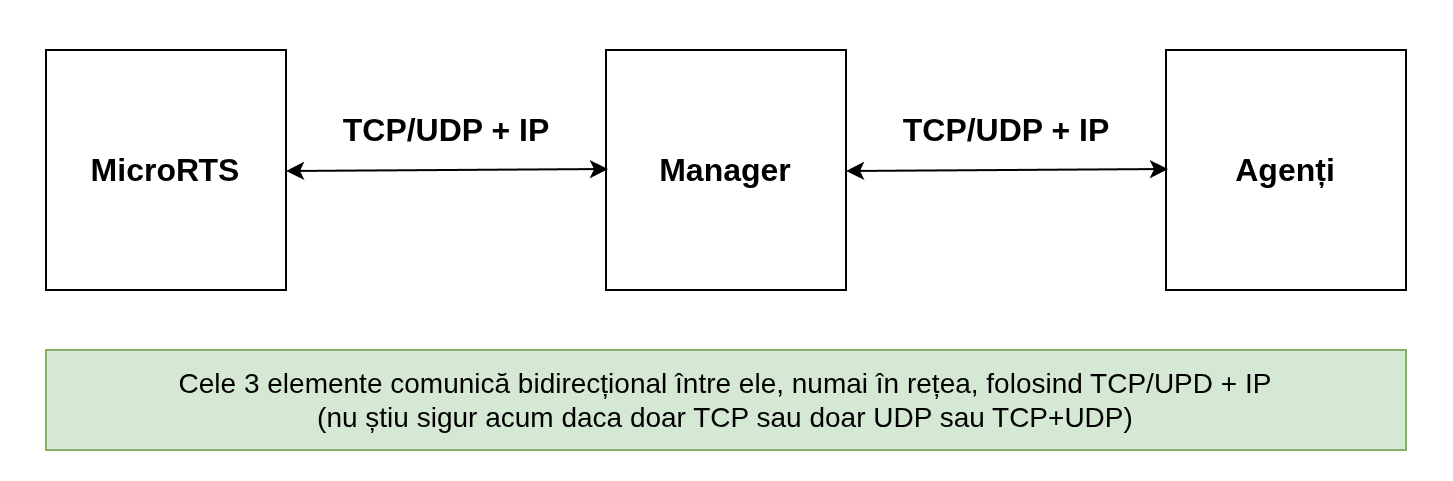
\includegraphics{ElementsCommunication.png}

Din cauza faptului că cele 3 elemente comunică între ele prin rețea(TCP/UDP + IP), putem avea mai multe instanțe de MicroRTS-Agenți, ele formând perechi.

Mai multe perechi MicroRTS-Agenti se pot conecta la același Manager pentru a rula, în paralel, mai multe experimente.

Instanțele de perechi MicroRTS-Agenți nu fac schimb de informații între ele.

Este un plan foarte ambition sa am multe instanțe de perechi MicroRTS-Agenți rulând în paralel. Este suficient să fac lucurile să meargă pentru o singură pereche MicroRTS-Agenți.

% E o imagine care descrie treaba asta, vezi MicroRTS-Agents_Pair_Multiple_Instances.png.


% Descrierea celor 3 elemente este aici, in acest enumerate.
% Doar descriere succinta, ideile de bază
\begin{enumerate}
\item \textbf{Jocul MicroRTS.}

Scurta Descriere MicroRTS

\item \textbf{Managerul}

Scurta Descriere Manager

\item \textbf{Agenții}

Scurta Descriere Agenti
\end{enumerate}

% Some ideas that i don't want to forget
%Aici e ideile mari boss
%uite niste idei noi:
%Suna misto:
%Win Condition/ Win conditions
%Constraints(constrangeri)
\end{document}